% figs/droplet_instability_tikz.tex
\documentclass[tikz,border=0pt]{standalone}
\usepackage{newtxtext,newtxmath}
\usetikzlibrary{arrows.meta,positioning,calc}
\tikzset{
  >=Latex,
  line/.style={line width=.8pt},
  % ドロップ
  drop/.style={draw,fill=white,circle,minimum size=3.4mm,line width=.8pt},
  sat/.style ={drop,minimum size=2.6mm},
  % ラベル(白背景で重なり防止)
  lbl/.style={font=\footnotesize,fill=white,inner sep=1pt,rounded corners=1pt}
}

\begin{document}
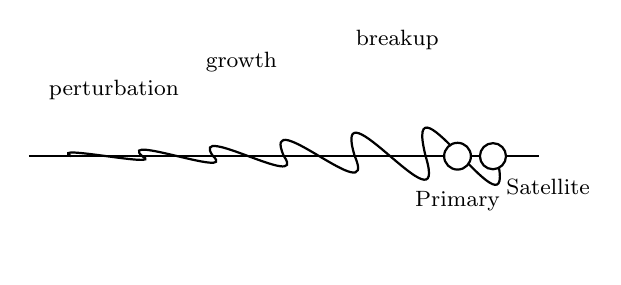
\begin{tikzpicture}[x=0.9cm,y=0.9cm]
  %--- jet axis
  \draw[line] (0,0) -- (7.2,0);

  %--- sinusoidal growth to breakup
  \foreach \x/\a in {0.6/0.18,1.6/0.32,2.6/0.50,3.6/0.80,4.6/1.15,5.6/1.40}{
    \draw[line] (\x,0) .. controls +(-0.35,\a) and +(0.35,-\a) .. (\x+1,0);
  }

  %--- callouts
  \node[lbl,above] at (1.2,0.75) {perturbation};
  \node[lbl,above] at (3.0,1.15) {growth};
  \node[lbl,above] at (5.2,1.45) {breakup};

  %--- main drop & satellite(座標固定)
  \node[drop] (main) at (6.05,0) {};
  \node[sat]  (sat)  at (6.55,0) {};

  %--- キャプション文字は“線と重ならない”ように y を下げる
  \node[lbl,below=2.2mm of main] {Primary};
  \node[lbl,below right=1.2mm and 0mm of sat] {Satellite};
\end{tikzpicture}
\end{document}
